%%% Appendix including ripple stuf %%%

\chapter{Open-loop ripple results}

The measurements and calculations of the current ripple and the voltage ripples are included in this section. Furthermore the section is divided in the simulation result and experiment result.
 \label{app:OL_ripple}
 
\section{Simulation}
The figures in this section shows the waveforms of the current and voltage ripples under worst case conditions. These conditions have been described during the calculations of the passive components in section \ref{component_sizing}. The maximum, minimum and mean values will be read and used to calculated the ripples in section \ref{opsimresult}. The data from the simulations have been loaded into Matlab to achieve accurate readings.

Figure \ref{fig:inductor_ripple} shows the current ripple in the inductor. The maximum and minimum currents are read as $I_{max} = 3.465A$ and $I_{min} = 3.135A$, with a mean at $\widebar{I_L} = 3.3A$.

Figure \ref{fig:output_voltage_ripple} shows the voltage ripple at the output capacitor. The maximum and minimum voltages are read as $V_{max} = 90.22V$ and $V_{min} = 89.77V$, with a mean at $\widebar{V_{out}} = 89.995V$.


\begin{figure}[H]
	\begin{minipage}[c]{0.5\textwidth}
		\centering
		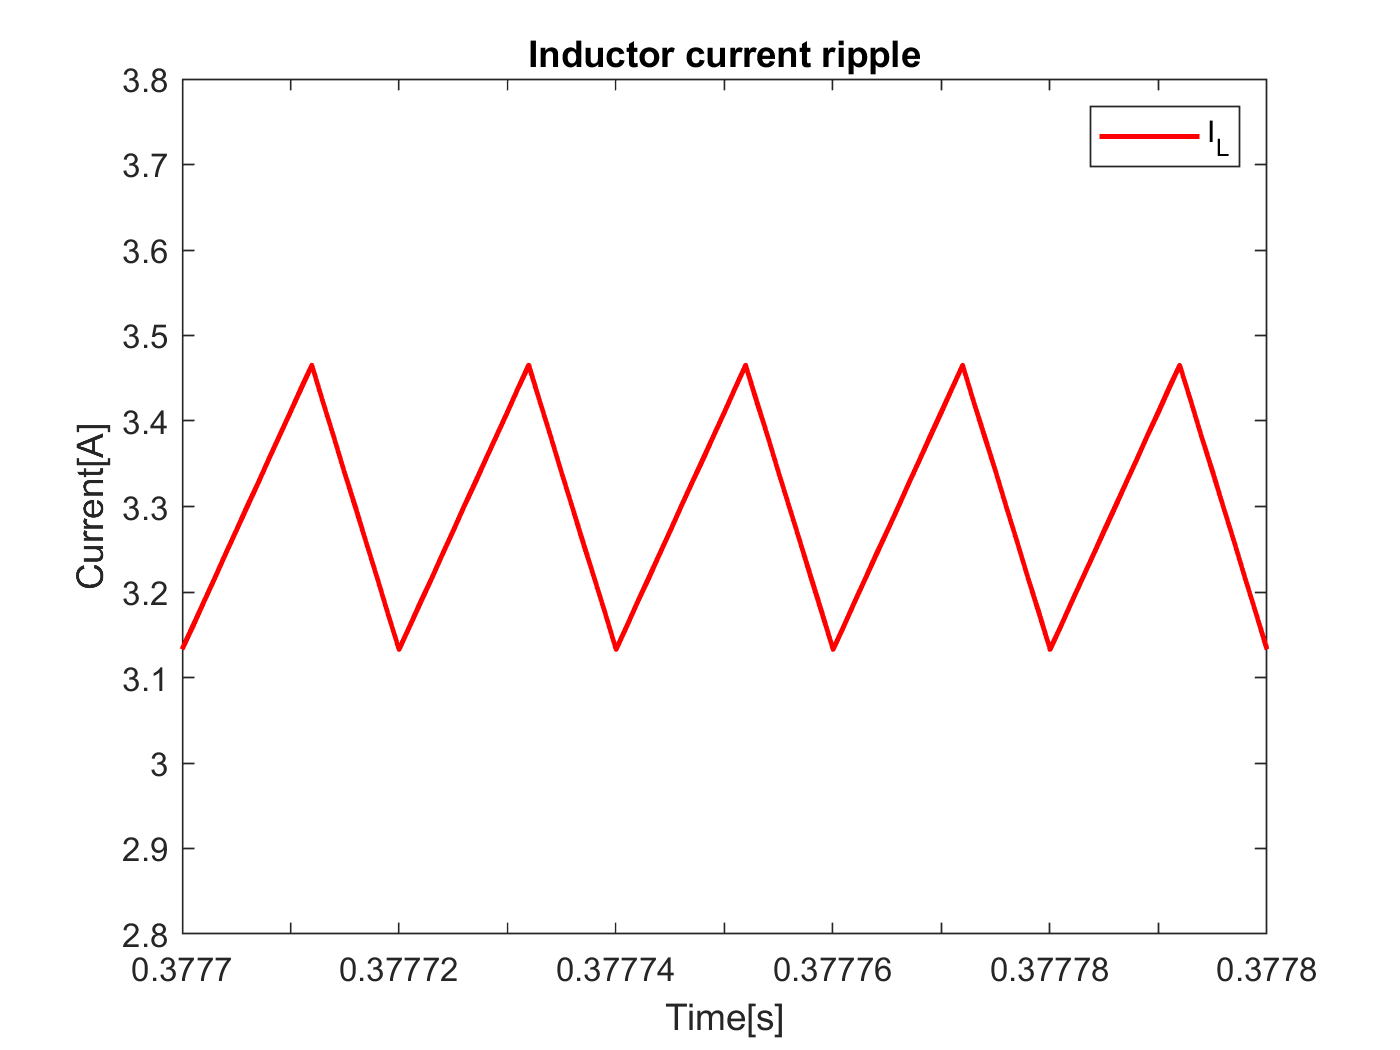
\includegraphics[width=1\textwidth]{../Pictures/P1/Open_loop_simulation/open_loop_IL_ripple} % Left picture
		\caption{Inductor current ripple.}
		\label{fig:inductor_ripple}
	\end{minipage}
	\hfill
	\begin{minipage}[c]{0.5\textwidth}
		\centering
		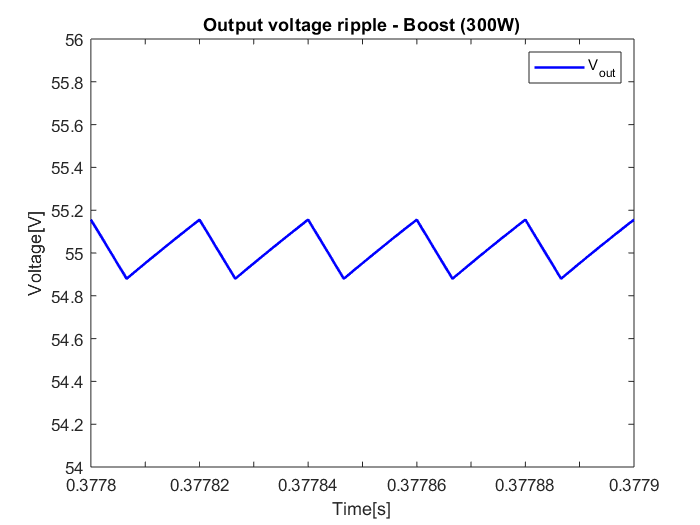
\includegraphics[width=1\textwidth]{../Pictures/P1/Open_loop_simulation/open_loop_Vout_ripple} % Right picture
		\caption{Output voltage ripple.}
		\label{fig:output_voltage_ripple}
	\end{minipage}  
\end{figure}

\section{Experiment}

The signal of the input capacitor voltage is noisy as you can see in figure \ref{Openlooptestinputcapacitor}. So it is not possible to measured the ripple.

\begin{figure}[H]
	\begin{center}
		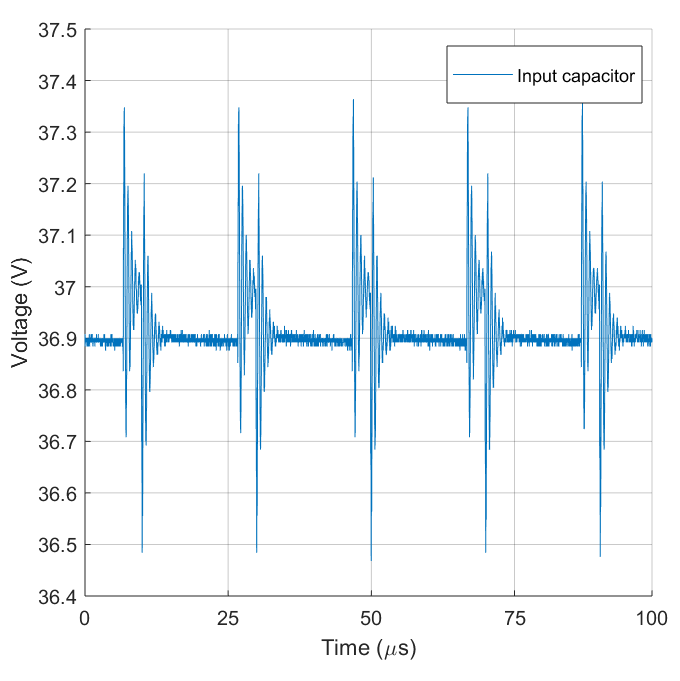
\includegraphics[width=0.5\textwidth]{../Pictures/P1/Test/Openloopinputcapacitor}
		\caption{Open-loop test: Input capacitor ripple.}
		\label{Openlooptestinputcapacitor}
	\end{center}	
\end{figure}

The figure \ref{Openlooptestoutputtcapacitor} presents the voltage ripple at the output capacitor. Because of the noise it is difficult to capture the exactly value for the maximum and minimum voltage from the triangle wave. For the equation \ref{eq:output_voltage_rippleexperiment} the values $V_{out,max} = 23.9082V$, $V_{out,min} = 23.895V$ and $\widebar{V_{out}} = 23.9V$ are used from the figure  \ref{Openlooptestoutputtcapacitor}.

\begin{figure}[H]
	\begin{center}
		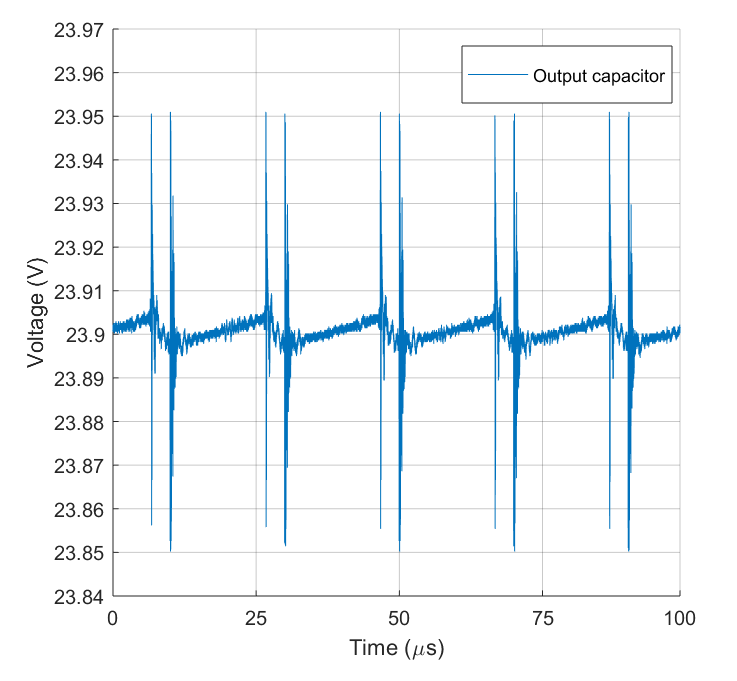
\includegraphics[width=0.5\textwidth]{../Pictures/P1/Test/Openloopoutputcapacitor}
		\caption{Open-loop test: Output capacitor ripple.}
		\label{Openlooptestoutputtcapacitor}
	\end{center}	
\end{figure}

The figure \ref{Openlooptestinductor} shows the current ripple at the inductor. From this figure it can be obtained  the minimum current $I_{min} = 2.7A$ and the maximum current $I_{max} = 2.98A$. The mean value for the inductor current is $\widebar{I_L}= 2.84$.

\begin{figure}[H]
	\begin{center}
		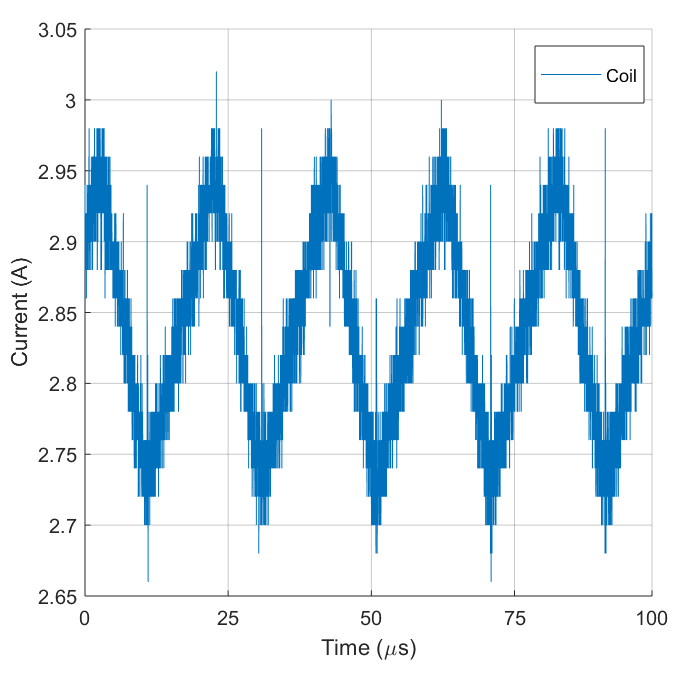
\includegraphics[width=0.5\textwidth]{../Pictures/P1/Test/Openloopinductor}
		\caption{Open-loop test: Inductor current ripple.}
		\label{Openlooptestinductor}
	\end{center}	
\end{figure}